\documentclass{TIJMUjiaoanSY}
\pagestyle{empty}


\begin{document}


%课程名称
\kecheng{Linux系统概论}
%实验名称
\shiyan{实验5\ Linux高级命令的操作}
%教师姓名
\jiaoshi{伊现富}
%职称
\zhicheng{讲师}
%教学日期(格式:XXXX年XX月XX日XX时-XX时)
\riqi{2018年6月4日13:30-15:30}
%授课对象(格式:XXX系XXXX年级XX班(硕/本/专科))
\duixiang{生物医学工程学院2016级生信班(本)}
%实验人数
\renshu{28}
%实验类型
\leixing{验证型}
%实验分组
\fenzu{一人一机}
%学时数
\xueshi{2}
%教材版本
\jiaocai{Linux系统概论上机指南(自编教材)}


%教案首页
\firstHeader
\maketitle
\thispagestyle{empty}

\mudi{
\begin{itemize}
  \item 了解datamash的使用方法。
  \item 了解Linux命令在生物信息学文本处理中的应用。
  \item 掌握find、grep、sed和AWK的使用方法。
\end{itemize}
}

\fenpei{
\begin{itemize}
  \item (10')元字符和正则表达式:回顾元字符和正则表达式的基础知识。
  \item (10')文本处理命令:通过实例回顾find、grep、sed和AWK的使用方法,总结常用的文本处理命令。
  \item (80')实验操作:以CentOS发行版为例,练习find、grep、sed和AWK等高级命令的使用,掌握它们的基本语法。
\end{itemize}
}

\cailiao{
\begin{itemize}
  \item 主要仪器:一台安装有CentOS的计算机。
\end{itemize}
}

\zhongdian{
\begin{itemize}
  \item 重点难点:正则表达式的构建,find、grep、sed和AWK的基本语法。
  \item 解决策略:通过实例进行讲解,通过演示进行学习,通过练习熟练掌握。
\end{itemize}
}

\sikao{
\begin{itemize}
  \item 列举常见的元字符并解释其含义。
  \item 根据要求构建正则表达式。
  \item 使用find、grep、sed和AWK完成指定的任务。
  \item 根据要求组合使用文本处理命令。
  \item 根据要求使用Linux命令处理生物信息学文本数据。
\end{itemize}
}

\cankao{
\begin{itemize}
  \item Linux基础及应用习题解析与实验指导(第二版),谢蓉\ 编著。中国铁道出版社,2014。
\end{itemize}
}

\firstTail


%教案续页
\newpage
\otherHeader

\noindent
\begin{enumerate}
  \item 元字符和正则表达式(10分钟)
%\parpic[fr]{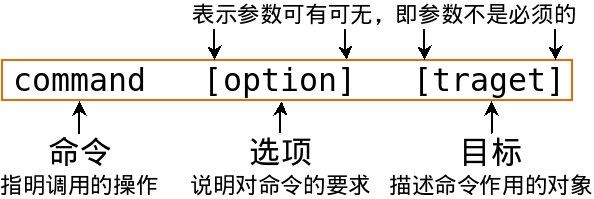
\includegraphics[width=8.5cm,height=2.3cm]{c4_command.png}}
    \begin{enumerate}
      \item 简介
	\begin{itemize}
	  \item 元字符:代表一组字符或命令的字符,用最小的字符集表示多组文本。
	  \item 正则表达式:具有一定句法的集合或短语,包含元字符或普通字符,表示某类文本或字符串。
	  \item 相关命令:less,more,grep,sed,AWK,vim,……
	\end{itemize}
      \item 元字符\textcolor{red}{(结合实例与完整的正则表达式讲解每一个元字符)}
	\begin{itemize}
	  \item 字符:一般字符,\verb|.|,\verb|[]|,\verb|[a-z]|,\verb|[0-9]|,\verb|[^]|,\verb|\|
	  \item 字符集:\verb|\d|,\verb|\D|,\verb|\s|,\verb|\S|,\verb|w|,\verb|\W|
	  \item 量词:\verb|?|,\verb|*|,\verb|+|,\verb|{m}|,\verb|{m,n}|
	  \item 边界:\verb|^|,\verb|$|
	  \item 其他:\verb|()|,\verb=|=
	\end{itemize}
	\vspace*{-8pt}
	\begin{figure}[h]
	  \centering
	  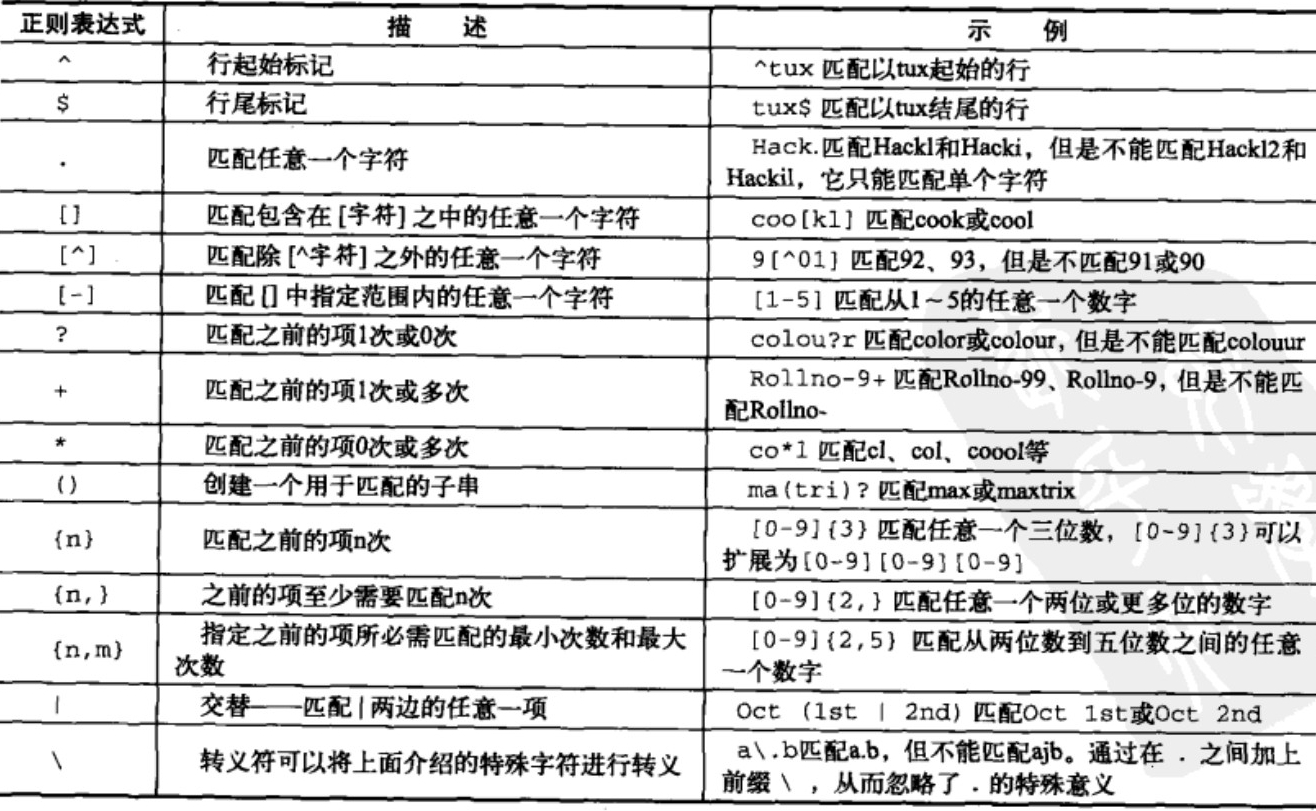
\includegraphics[width=16cm]{c5_meta_03.jpg}
	\end{figure}
	\vspace*{-8pt}
      \item 正则表达式
	\vspace*{-8pt}
	\begin{figure}[h]
	  \centering
	  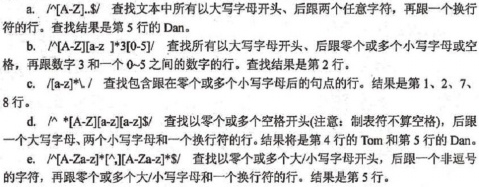
\includegraphics[width=16cm]{c5_re_example_02.jpg}
	\end{figure}
	\vspace*{-8pt}
    \end{enumerate}

\otherTail
\newpage
\otherHeader

  \item 文本处理命令(10分钟)
    \begin{enumerate}
      \item find\textcolor{red}{(通过实例讲解find的语法和使用)}
	\begin{figure}[h]
	  \centering
	  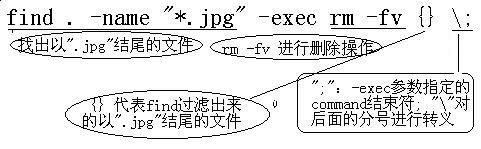
\includegraphics[width=16cm]{c5_find_02.jpg}
	\end{figure}
      \item grep\textcolor{red}{(通过实例讲解grep的语法和使用,注意正则表达式在其中的应用)}
	\begin{figure}[h]
	  \centering
	  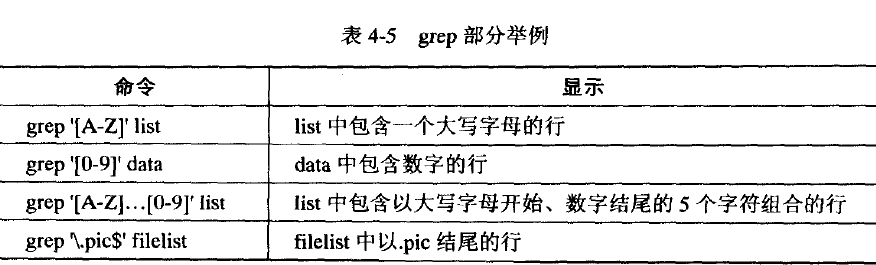
\includegraphics[width=16cm]{c5_grep_02.png}
	\end{figure}
      \item sed\textcolor{red}{(通过实例讲解sed的语法和使用)}
        \begin{itemize}
          \item \verb|sed -n '1,3!p' 123.txt|
          \item \verb|sed -n -e '/the/p' -e '/the/=' 123.txt|
          \item \verb|sed 's/this/that/g' 123.txt|
          \item \verb=echo "hello" | sed 's/$/.txt/g'=
          \item \verb=ls -l | sed -n '1,3p'=
        \end{itemize}
      \item AWK\textcolor{red}{(通过实例讲解AWK的语法和使用)}
        \begin{itemize}
          \item \verb|awk '{print $0}' 123.txt|
          \item \verb=ls -l | awk '{if($1 !~ /^d/) {print $0}}'=
          \item \verb|awk '{printf("%03d %s\n",NR,$0)}' ori.txt > dst.txt|
          \item \verb|awk 'BEGIN{FS=" ";OFS="\t"}{print $1,$2} ori.txt > dst.txt|
        \end{itemize}
      \item 文本处理命令
	\begin{enumerate}
	  \item 常用文本处理命令\\
	    cut,sort,uniq,split,paste,join,comm,tr,……
	  \item 使用实例
	    \begin{figure}[h]
	      \centering
	      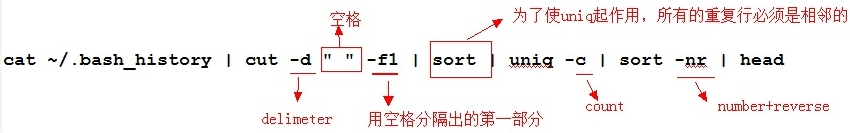
\includegraphics[width=17cm]{c5_text_02.jpg}
            \end{figure}
	\end{enumerate}
    \end{enumerate}

\otherTail
\newpage
\otherHeader

  \item 实验操作(80分钟)
    \begin{enumerate}
      \item find的使用
	\begin{enumerate}
	  \item 根据文件名查找文件:-name,-iname
	  \item 限定搜索目录的深度:-maxdepth,-mindepth
	  \item 在找到的文件上执行命令\textcolor{red}{(理解基本的语法,-exec vs. -ok)}
	  \item 相反匹配:-not
	  \item 根据inode查找文件:-inum
	  \item 根据文件权限查找文件:-perm,-type
	  \item 查找空文件:-empty
	  \item 查找最大最小的文件\textcolor{red}{(组合使用find、sort和head)}
	  \item 查找指定类型的文件:-type
	  \item 根据文件大小查找文件:-size,+,-
	  \item 根据时间戳查找文件:-mmin,-mtime,-amin,-atime,-cmin,-ctime
	  \item 基于文件比较进行查找:-newer,-anewer,-cnewer
	\end{enumerate}
      \item grep的使用\textcolor{red}{(常用选项:-i,-v,-A,-B,-C,-c,-n,-w,-f)}
      \item sed的使用\textcolor{red}{(常用选项与命令:-e,-f;s,d)}
      \item AWK的使用\textcolor{red}{(基本语法结构,字段的含义)}
      \item datamash的使用\textcolor{red}{(学生课后自学,与AWK、Perl、R等进行比较)}
    \end{enumerate}
\end{enumerate}


\otherTail


\end{document}

